\section{USGS ScienceBase}

To facilitate and encourage data sharing and dissemination, 
the U.S. Geological Survey has created ScienceBase, an online 
collaborative scientific data platform (Figure \ref{fig:sbfig}). To support collaborative 
data workflows, ScienceBase has four key elements. 1) Data and metadata
cataloging and hosting with options for private, controlled access 
and fully public sharing of data and metadata. 2) Central search and
data discovery including metadata search for linked, non-hosted data. 
3) Full web-service support for all core functionality, including 
standards-based access to specific data types (e.g., Geospatial 
datasets). 4) Research community catalogs to 
enable the organization of data along collaborative group and 
organizational boundaries. 

 \begin{figure}[htbp]
   \centering
   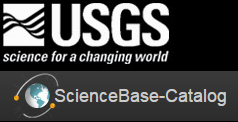
\includegraphics{sblogo}
   \caption{The ScienceBase platform logo}
   \label{figure:sbfig}
 \end{figure}

ScienceBase functionality revolves around the organization of data 
items in a hierarchical structure. These items are flexible representations
of a single dataset with metadata attached. ScienceBase can be used to
store the raw data with attached metadata, or be only the metadata 
repository with links to external data repositories. These data items
are organized into a tree hierarchy (much like the organization of files
on a hard drive). This makes the organization of data by collaborative 
group, project, and/or individual data owner simple. 

Search and access of ScienceBase data items can be accomplished through
a variety of useful interfaces. For manual search and data editing, 
the ScienceBase website offers full functional interfaces. Automated
access is supported by robust REST-ful web services that support all 
functionality offered by the human interfaces. 

The ScienceBase code and infrastructure setup is available upon 
request from the ScienceBase team <sciencebase@usgs.gov>.

